\section{Acceptance Sampling}
\noindent\rule[\linienAbstand]{\linewidth}{\linienDickeDick}
Acceptance control is based on acceptance sampling plans, which contain instructions based on which the acceptance or return of a lot is decided.\\
We should remember that the actual point of acceptance control is not to value quality, but to decide whether or not delivery will likely pass quality control.

\textbf{Idea:} Draw random samples from a lot and make a decision on the quality of the lot based on this information.

\subsection{Plans for Attributes}
\noindent\rule[\linienAbstand]{\linewidth}{\linienDicke}
\textbf{Percent defective}\\
We have a lot of N parts (known). The number of defective parts m (unknown) with $0 \leq m \leq N$ is observed. Thus, the percent defective is:
\begin{equation}
  p = \frac{m}{N}
\end{equation}

\textbf{Acceptance sampling plan} consitst of:\\
 - Sample size n,\\
 - the number of defective parts x in the sample, where $0 \leq x < n$,\\
 - the acceptance number c, where $0 \leq c < n$ and\\
 - the rule: if $x \leq c$, then the lot is accepted, if $x > c$, then the lot is rejected.\\

\textbf{Hypothesis test}\\
The rule above can also be formulated as a hypothesis test:
\begin{equation}
  \begin{split}
    H_0:& x \leq c,\text{ i.e. the lot is not rejected.}\\
    H_1:& x > c,\text{ i.e. the lot is rejected.}\\
  \end{split}
\end{equation}

As with any hypothesis test the following two errors can be made.\\

\textbf{Type I Error}\\
$H_0$ true, but rejected (Lot is good but is rejected)\\
Probability for this to happen (false negative): $\alpha$. (Producer's risk)\\
The producer wants to avoid type I error, i.e. does not want good lots to be returned.\\

\textbf{Type II Error}\\
$H_0$ false, but accepted (Lot is bad but is accepted)\\
Probability for this to happen (false positive): $\beta$. (Consumer's risk)\\
The consumer wants to avoid type II error, i.e. does not want to accept bad lots.\\


In an agreement between a producer and a consumer the following parameter must de defined:\\
- $\alpha$: The producer's acceptable probability of falsly rejecting a good lot,\\
- $\beta$: The consumer's acceptable probability of falsly accepting a bad lot,\\
- $p_{\alpha}$ the producer's minimal percentage defective needed for a lot to be returned (The producer does not want to take back lots with $p < p_{\alpha}$.),\\
- $p_{\beta}$ the consumer's maximal percentage defective needed for a lot to be accepted (The consumer wants to reject lots with $p_{\beta} < p$ whenever possible).

\subsection{Operating Characteristic}
\noindent\rule[\linienAbstand]{\linewidth}{\linienDicke}
The operating characteristic, short OC, is the probability of accepting a lot as a function of the percent defective p.\\
The number of defective units X is a hypergeometric random variable. There are N parts in total, among which m defective and N - m are good parts. So a sample of size n is drawn at once. The probability that among these n parts are at most c parts defective is given by
\begin{equation}
  OC(p) = P(X \leq c)= \sum^c_{k=0} P(X = k) = \sum^c_{k=0} \frac{\binom{pN}{k}\binom{N-pN}{n-k}}{\binom{N}{n}}
\end{equation}
For a given lot size N, the parameters n and c of the acceptance sampling plan determine the form of the OC curve.\\

\textbf{Ideal OC Curve}\\
If all parts of a lot get checked we get an ideal acceptance sampling plan:
\begin{figure}[H]
  \centering
  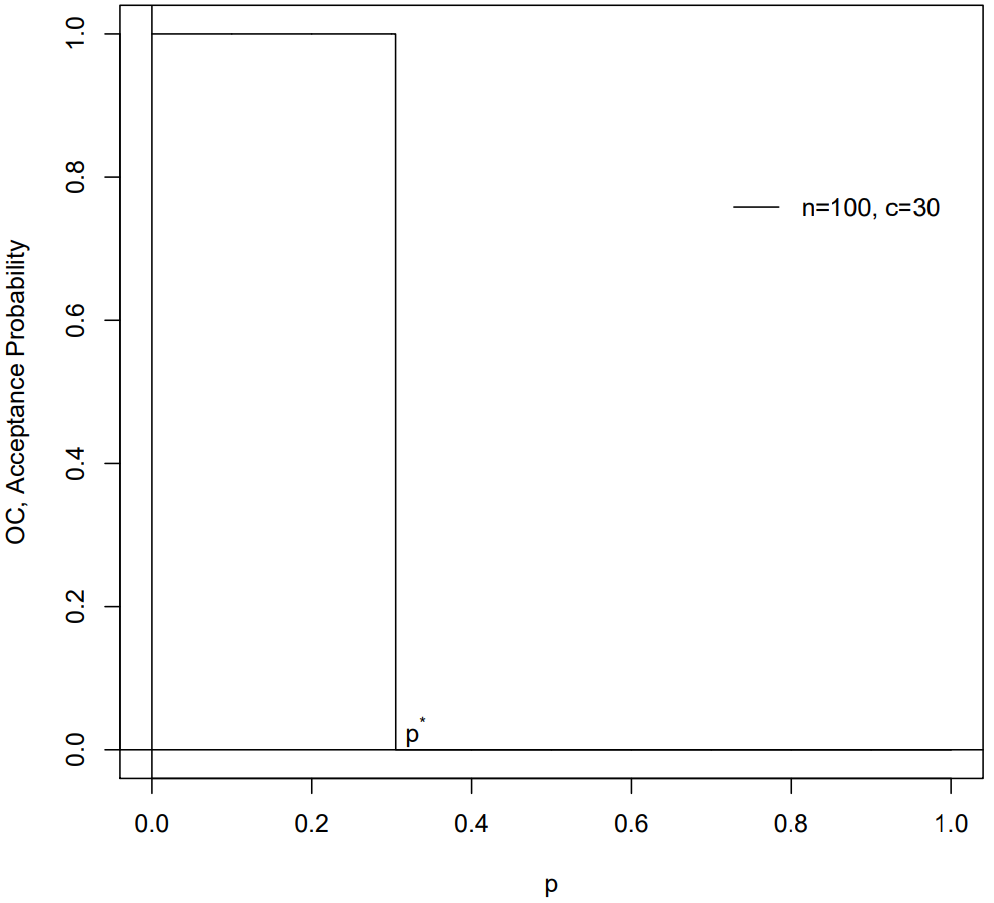
\includegraphics[width=0.8\linewidth]{Pics/5.1.1.png}
  \caption{OC curve of an ideal acceptance sampling plan}
\end{figure}

\textbf{OC Curves - Examples}
\begin{figure}[H]
  \centering

  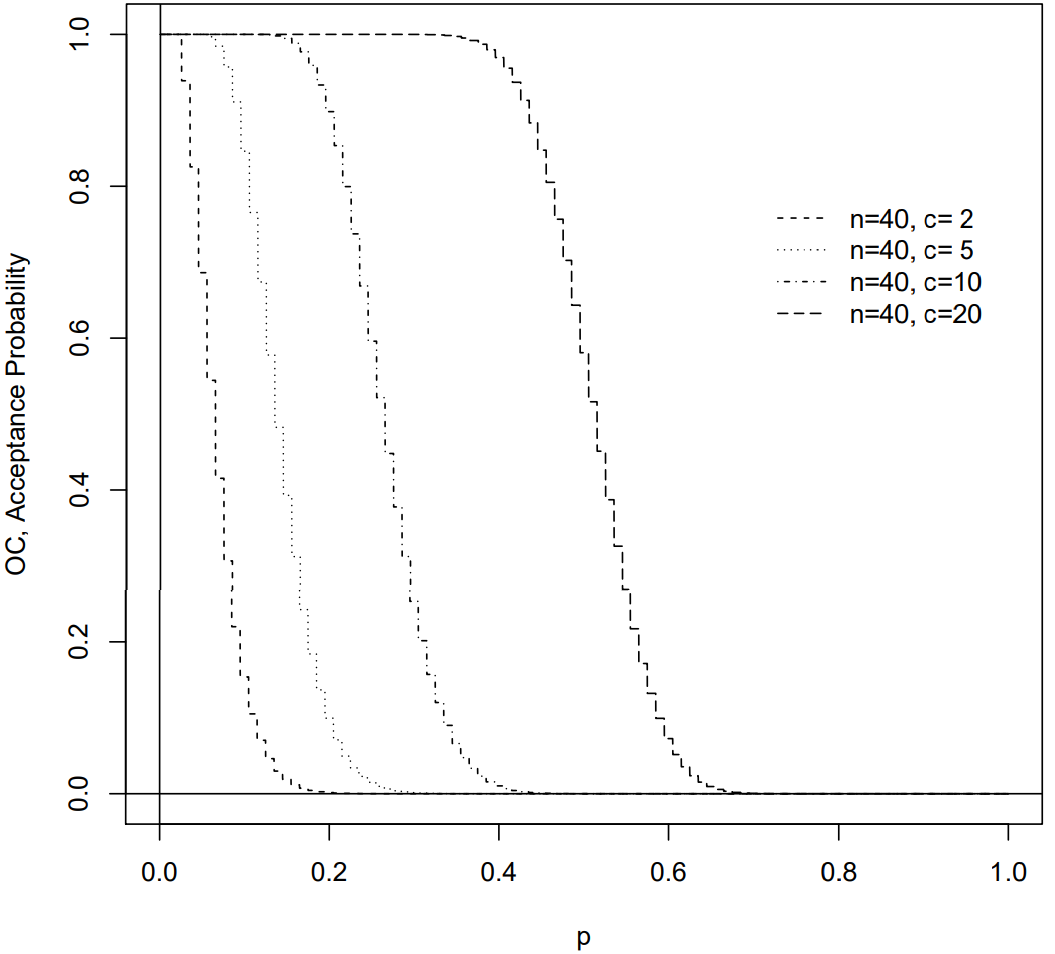
\includegraphics[width=0.8\linewidth]{Pics/5.1.2.png}
  \caption{OC curve with fixed n and increasing c}
\end{figure}

\begin{figure}[H]
  \centering
  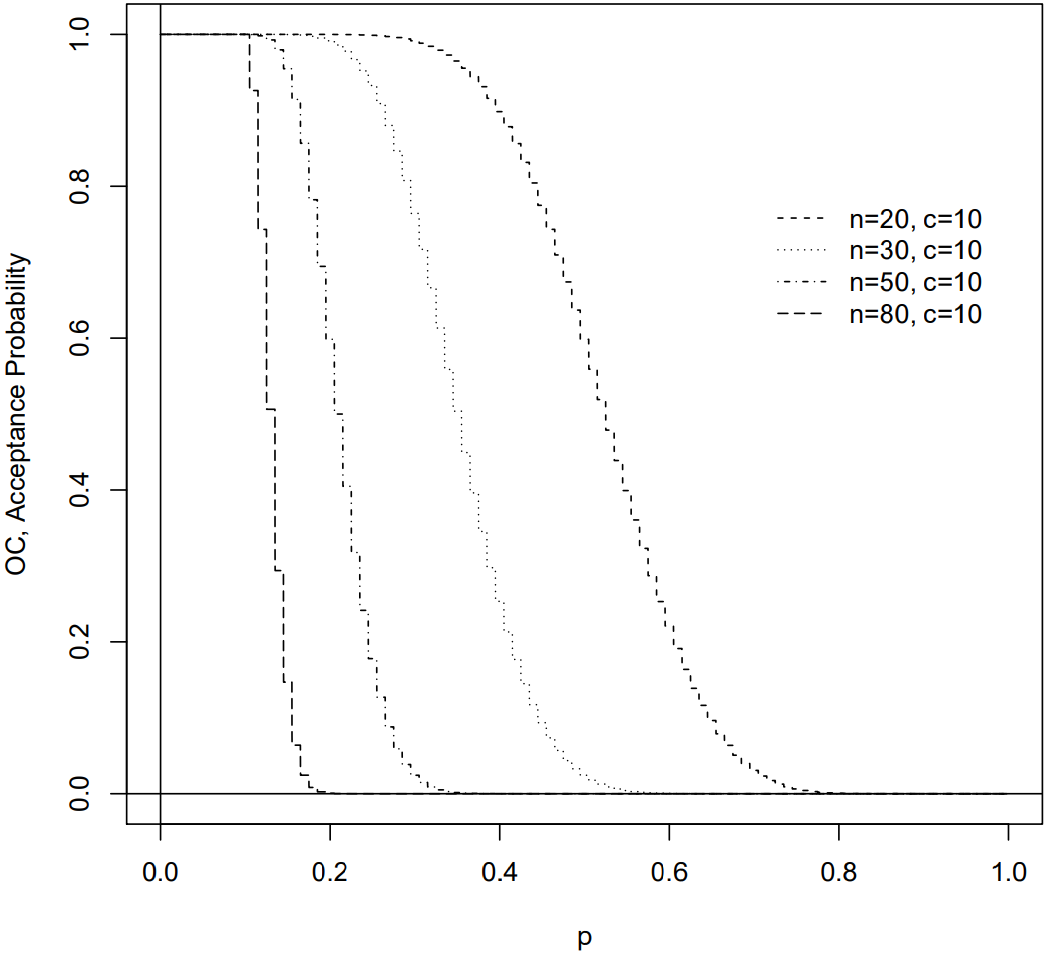
\includegraphics[width=0.8\linewidth]{Pics/5.1.3.png}
  \caption{OC curve with increasing n and fixed c}
\end{figure}

\subsection{Parameters of an Acceptance Sampling Plan}
\noindent\rule[\linienAbstand]{\linewidth}{\linienDicke}
n and c are to be chosen such that:\\
- n is as small as possible,\\
- the producer risk is at most equal to $\alpha$, i.e. $OC(p_{\alpha}) \leq 1 - \alpha$, and\\
- the consumer risk is at most equal to $\beta$, i.e. $OC(p_{\beta}) \geq \beta$\\

The pair $(p_{\alpha}, 1-\alpha)$ is called producer risk point and the pair $(p_{\beta}, \beta)$ is called consumer risk point.\\
n and c are calculated by brute force. The resulting OC curve is not a perfect fit since only integer values can be choosen.\\

\textbf{Real OC Curve}
\begin{figure}[H]
  \centering
  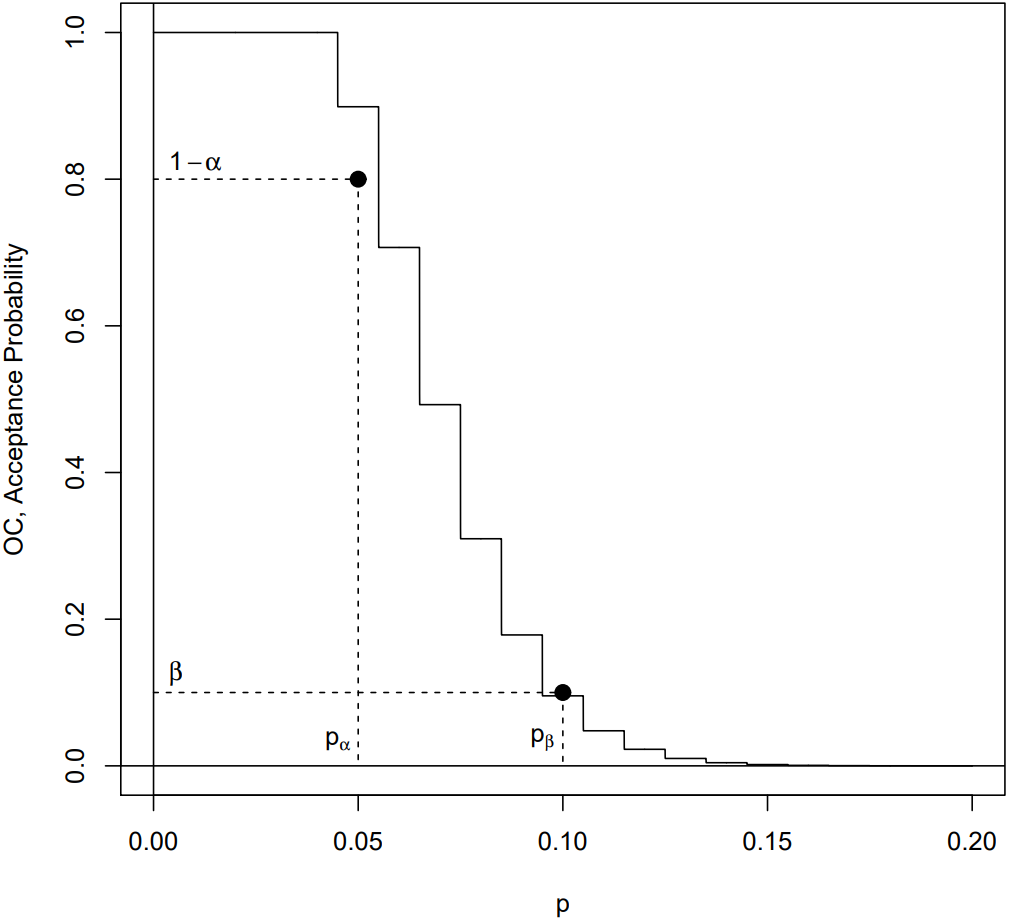
\includegraphics[width=0.8\linewidth]{Pics/5.1.4.png}
  \caption{OC curve of a real acceptance sampling plan.}
\end{figure}


\subsection{Acceptance Sampling Plans for Variables}
\noindent\rule[\linienAbstand]{\linewidth}{\linienDicke}
It is always possible to reduce an acceptance sampling plan for variables to an acceptance sampling plan for attributes by saying:\\

- If $LSL \leq x \leq USL$, then the part is fit for use.\\
- If $x < LSL \text{ or } USL < x$, then the part is rejected\\

By counting the number of rejected parts, we again have an acceptance sampling plan for attributes.
